\documentclass[letterpaper,final,12pt,reqno]{amsart}

\usepackage[total={6.3in,9.2in},top=1.1in,left=1.1in]{geometry}

\usepackage{bm}
\usepackage{empheq}
\usepackage[dvipsnames]{xcolor}
\usepackage{graphicx}
\usepackage{verbatim,fancyvrb}
\usepackage{tikz}
\usepackage{times}

% hyperref should be the last package we load
\usepackage[pdftex,
colorlinks=true,
plainpages=false, % only if colorlinks=true
linkcolor=blue,   % only if colorlinks=true
citecolor=Red,   % only if colorlinks=true
urlcolor=black     % only if colorlinks=true
]{hyperref}

\renewcommand{\baselinestretch}{1.05}

\newcommand{\ddt}[1]{\ensuremath{\frac{\partial #1}{\partial t}}}
\newcommand{\ddx}[1]{\ensuremath{\frac{\partial #1}{\partial x}}}
\newcommand{\ddy}[1]{\ensuremath{\frac{\partial #1}{\partial y}}}
\newcommand{\pp}[2]{\ensuremath{\frac{\partial #1}{\partial #2}}}
\renewcommand{\t}[1]{\texttt{#1}}
\newcommand{\Matlab}{\textsc{Matlab}\xspace}
\newcommand{\eps}{\epsilon}
\newcommand{\RR}{\mathbb{R}}

\newcommand{\grad}{\nabla}
\newcommand{\Div}{\nabla\cdot}
\newcommand{\trace}{\operatorname{tr}}

\newcommand{\hbn}{\hat{\mathbf{n}}}

\newcommand{\bg}{\mathbf{g}}
\newcommand{\bn}{\mathbf{n}}
\newcommand{\bu}{\mathbf{u}}
\newcommand{\bv}{\mathbf{v}}
\newcommand{\bx}{\mathbf{x}}

\newcommand{\bV}{\mathbf{V}}
\newcommand{\bX}{\mathbf{X}}

\newcommand{\bxi}{\bm{\xi}}

\newcommand{\bzero}{\bm{0}}

\newcommand{\Href}{H_{\text{ref}}}

\newtheorem{lemma}{Lemma}


\begin{document}
\title[Performance of evolving-geometry glacier flow simulations]{Performance of evolving-geometry glacier flow simulations using Stokes dynamics}

\author{Ed Bueler}

\maketitle

\thispagestyle{empty}
\bigskip

\section{Introduction} \label{sec:intro}

The most important questions in glaciology concern how the climate around a glacier determines its geometry, both through internal dynamics and through changes in the climate along the ice surface.  The relationship between surface mass inputs and the geometry of the ice mass is important because it affects sea level, deformations of the Earth's crust, and fresh water supplies for people, among other concerns.  As a result, evolving-geometry simulations are widely used by scientists to understand the size and extent of glaciers and ice sheets.

A variety of methodologies for such numerical simulations are used in practice, with most of the well-established schemes involving shallowness approximations in the continuum equations \cite[for example]{Hoffmanetal2018,Lipscombetal2019,Winkelmannetal2011}.  Furthermore, most methods use explicit or semi-implicit time-stepping, with correspondingly small time steps at high spatial resolution, though fully-implicit exceptions exist \cite{Brinkerhoffetal2017,Bueler2016}.  The performance properties of current numerical models tend to limit either the physical modeling authenticity (due to shallowness and other approximations) or the spatial resolution (due to time-stepping and solver performance limitations).  In particular, the quality of ensemble simulations, regarding both the number of ensemble members and the quality of the individual simulations, is directly limited by numerical model performance.

This paper\footnote{version: \today} addresses an important, but also restricted, class of numerical glacier and ice sheet models which are based on the conservation of momentum and mass within the ice.  For conservation of momentum we use the standard shear-thinning (Glen) power-law Stokes model.  Noting that ``mass conservation'' properly refers both to fluid incompressibility and to conservation at the ice surface, we solve both the divergence-free equation for bulk ice and the surface kinematical equation (or kinematic boundary condition \cite{GreveBlatter2009}) wherein the surface mass balance is an input.  We model three-dimensional (3D) grounded glaciers and ice sheets for which there is a well-defined ice thickness---overhanging ice is thus not modeled---but with an evolving free boundary at the ice margin \cite{SchoofHewitt2013} (Figure \ref{fig:cartoon}).  The ice thickness is defined at all map-plane points but it is zero in those locations where the (coupled and solved) surface balance and ice flow do not determine the presence of glacier ice.

\begin{figure}[h]
\begin{center}
\includegraphics[width=0.7\textwidth]{cartoon.pdf}
\end{center}
\caption{We consider 3D models of grounded glaciers and ice sheets which are based on Glen-Stokes ice flow, an evolving free surface, and a free boundary.}
\label{fig:cartoon}
\end{figure}

We do not, however, consider the conservation of energy, that is, thermomechanical coupling or basal melt.  A further restriction is that our ice sticks to the bed (no slip), and we do not consider floating ice or otherwise sliding bases.  Finally we only consider cases where the bed elevations are relatively-smooth.  These restrictions are all removable by well-known modeling mechanisms \cite[for example]{Aschwandenetal2012,Winkelmannetal2011}, but how these components affects model performance is a topic for further research.

To discretize the continuum equations we apply the finite element (FE) method \cite{Elmanetal2014} by using the Firedrake library \cite{Rathgeberetal2016} in Python.\footnote{These Python programs are open-source at \href{https://github.com/bueler/stokes-implicit}{\texttt{github.com/bueler/stokes-implicit}}.  FIXME: MAKE REPO PUBLIC.}  We use meshes which are unstructured in the map-plane but which are extruded \cite{Gibsonetal2019}, thus structured, in the vertical direction.  As discussed below, mixed elements for velocity, pressure, and vertical ice strain are used, with stable and aspect-ratio robust choices for the velocity-pressure (i.e.~Stokes) block \cite{Elmanetal2014}.  Solutions of the resulting nonlinear discrete equations will use multigrid-preconditioned Newton-Krylov methods \cite{Bueler2021} via PETSc \cite{Balayetal2020}, and all computations are parallelized.

The model performance metric introduced here is a natural one for glacier modeling.  Namely, we measure the run time of coupled Glen-Stokes simulations relative to the well-understood computation of ice velocity in the shallow ice approximation (SIA) \cite{Fowler1997} on the same mesh.  That is, we define a glacier model ``work unit'' as the time needed for a diagnostic computation of the Glen-law SIA velocity solution, a trivialized PDE solution which only evaluates powers and does a vertical integration \cite{SchoofHewitt2013}.

The primary purpose of the paper is to understand the performance characteristics of numerical simulations using fully-implicit time-stepping with the above type of physical model.  That is, at each time step the Glen-Stokes momentum and surface kinematical equations are solved to a tolerance on the coupled residual.  Only the interaction between ice surface elevation and the evaluation of surface mass balance is split in time, and time steps of order one year are assumed.  To evaluate our approach we validate the model based on results of laboratory-scale experiments, compare the performance of the model with shallow models, demonstrate solver optimality and scalability, and show a solution for the Greenland ice sheet.


\section{Equations for ice flow in glaciers} \label{sec:strongform}

The standard model for the flow of glaciers uses Stokes equations based upon Glen's shear-thinning flow law for ice \cite{GreveBlatter2009,JouvetRappaz2011,SchoofHewitt2013}.  We will apply this model on time-dependent $d=2$ or $d=3$ dimensional domains using time $t>0$ and spatial variables $\bx=(x,y,z)$, with $z$ vertical.  (Coordinates are denoted $(x,z)$ in 2D.)  The evolving domain $\Omega^t \subset \RR^d$ will have a piecewise smooth boundary, so that we may apply the boundary conditions, but it is otherwise general.

Allowing any Glen exponent $n\ge 1$, the strong-form model equations are:
\begin{align}
- \nabla \cdot \tau + \nabla p &= \rho \bg &&\text{\emph{stress balance}} \label{forcebalance} \\
\nabla \cdot \bu &= 0 &&\text{\emph{incompressibility}} \label{incompressible} \\
\tau &= B_n |D\bu|^{(1/n) - 1} D\bu  &&\text{\emph{flow law}} \label{viscflowlaw}
\end{align}
The solution fields are velocity $\bu$, pressure $p$, and deviatoric stress tensor $\tau$.  For simplicity we take the ice density $\rho$ and the acceleration of gravity $\bg=\left<0,0,-g\right>$, with $g>0$, to be constant.

Regarding tensors and their notation, the full (Cauchy) stress tensor $\sigma$ decomposes into the deviatoric part $\tau$ minus the pressure, i.e.~$\sigma = \tau - p\,I$, so equation \eqref{forcebalance} simply says $-\Div \sigma = \rho \bg$.  The strain rate tensor $D\bu$ is the symmetric part of $\grad \bu$, i.e.~$(D\bu)_{ij} = \frac{1}{2} \left(\grad\bu + \grad\bu^\top\right)$.  Because $D\bu$ is symmetric, and because it has trace zero by equation \eqref{incompressible}, i.e.~$\trace(D\bu)=\nabla \cdot \bu = 0$, from equation \eqref{viscflowlaw} it follows that $\tau$ is also symmetric with trace zero.  The tensor norm in \eqref{viscflowlaw} satisfies $|D\bu|^2 = \frac{1}{2} \trace\left((D\bu)^2\right) = \frac{1}{2} (D\bu)_{ij} (D\bu)_{ij}$.  Note $B_n$ is the $n$-dependent ice hardness in units $\text{Pa}\,\text{s}^{1/n}$, sometimes written $B_n = (A_n)^{-1/n}$ in terms of the softness $A_n$.

For the linear Stokes equations \cite{Elmanetal2014}, i.e.~the $n=1$ case, one would traditionally write the flow law \eqref{viscflowlaw} as $\tau = 2\nu D\bu$, and in that case the viscosity would be $\nu = (1/2) B_1$.  However, for realistic powers $n>1$, namely shear-thinning ice, one defines an ``effective viscosity'' in equation \eqref{viscflowlaw} which involves a negative power of the strain rate magnitudes $|D\bu|$.  This effective viscosity is singular in the limit of small strain rates, and so, motivated by the expected finite viscosity of glacier ice \cite{GreveBlatter2009}, and noting the equations using regularized viscosity are well-posed \cite{JouvetRappaz2011}, we define the regularized effective viscosity
\begin{equation}
\nu_\eps(|D\bu|) = (1/2) B_n \left(|D\bu|^2 + \eps\, D_0^2\right)^{(r-2)/2} \label{regeffvisc}
\end{equation}
where $\eps = 0.0001$, $D_0 = 2 a^{-1}$, and $r=(1/n)+1$.  The constant $D_0$ defines a strain-rate scale for glacier flow; the value here corresponds to a velocity difference of 1000 meters per year in a distance of 500 meters.

Using \eqref{viscflowlaw}, as modified by \eqref{regeffvisc}, we eliminate $\tau$ from equation \eqref{forcebalance}, thereby rewriting the system in terms of velocity and pressure derivatives only:
\begin{align}
- \nabla \cdot \left(2 \nu_\eps(|D\bu|)\, D\bu\right) + \nabla p &= \rho \mathbf{g} \label{stokes} \\
\Div \bu &= 0 \label{incompagain}
\end{align}
This system is our Glen-Stokes model for bulk ice motion.  A solution is a velocity-pressure pair $(\bu,p)$, from which one may derive strain rates $D\bu$ and stresses $\tau$ and/or $\sigma = \tau - p\,I$.

Glacier-suitable dynamic boundary conditions will be used, with an emphasis on isolated, grounded glaciers.  In such cases the ice flow extends in the horizontal direction until a free boundary at the glacier margin is reached.  (In real glaciers grounded margins may occur as fracture-generated cliffs, but such non-fluid processes are not modeled here.)  As noted in the Introduction, we assume that the ice thickness is well-defined and thus that the top and bottom boundaries of $\Omega^t$ can, at each time, be identified, and that the ice base has positive measure.  On the top surface we set a condition of zero applied stress,
\begin{align}
\left(2 \nu_\eps(|D\bu|) D\bu - pI\right) \bn &= \bzero  &&\text{\emph{top}: } \overline{\partial} \Omega^t \label{topbc} \\
\intertext{where $\bn$ is normal to the surface.  On the base we require no slip:}
\bu &= \bzero  &&\text{\emph{base}: } \underline{\partial} \Omega^t \label{basebc} \\
\intertext{Optionally, to allow simulation of a certain laboratory experiment \cite{SayagWorster2013}, we also allow an inflow boundary on which a prescribed velocity $\bu_{\text{in}}$ is applied, subject to $\bu_{\text{in}}\cdot \bn \le 0$ where $\bn$ is an outward normal:}
\bu &= \bu_{\text{in}}  &&\text{\emph{inflow}: } \partial_{\text{in}} \Omega^t. \label{inflowbc}
\end{align}

Assuming the well-posedness of the above model \eqref{stokes}--\eqref{inflowbc}, as is proven by \cite{JouvetRappaz2011}, if the ice geometry $\Omega^t$ is known then the solution is a unique pair $(\bu,p)$.  Note that the slowness of the fluid, i.e.~zero Reynolds number, implies that the given boundary stresses and body forces determine velocity and pressure fields without any ``memory'' of prior states or influence from inertia, as would arise in the Navier-Stokes equations \cite{Fowler1997}.


\section{Ice geometry and its evolution} \label{sec:stronggeometry}

The above equations do not describe how the glacier changes shape or extent.  This process, which is coupled to the ice flow but not fully determined by it, is described by an additional equation which states conservation of mass on the top boundary $\overline{\partial} \Omega^t$.  To present this equation we first assume a larger map-plane computational domain $R\subset \RR^{d-1}$ on which the input surface mass balance and bedrock elevation data of the problem are defined; see Figure \ref{fig:domainnotation}.  The ice-covered area is then a subset of the interior of $R$; that is, we require that ice is not present on, nor does it flow across, the boundary of $R$.

Let $z=b(x,y)$ be the bedrock elevation, assumed continuously-differentiable and time-independent for simplicity, and $z=h(x,y,t)$ be the ice surface elevation; note that both functions are defined for all $(x,y)\in R$.  The surface elevation function, a part of the solution, will be continuous and smooth.  The following time-dependent form for the (open) ice domain is now assumed:
\begin{equation}
\Omega^t = \left\{\bx\,\big|\,(x,y)\in R \,\text{ and }\, b(x,y) < z < h(x,y,t)\right\}.  \label{Omegat}
\end{equation}
An admissibility requirement \cite{Bueler2016} for $h$, as a part of the model solution, is that at each $t>0$ and $(x,y)\in R$ we have
\begin{equation}
h(x,y,t) \ge b(x,y).  \label{admissibility}
\end{equation}
That is, at a given map-plane location $(x,y)$ the ice may be present (strict inequality in \eqref{admissibility}) or absent (equality) in an evolving, time-dependent manner.  The time-dependent ice-covered map-plane domain, the vertical projection of $\Omega^t$, is denoted $\pi \Omega^t$.

\begin{figure}[h]
\begin{center}
\includegraphics[width=0.7\textwidth]{domainnotation.pdf}
\end{center}
\caption{Notation: The evolving ice domain $\Omega^t$ has projection $\pi \Omega^t$.  Surface mass balance $a$ and bedrock elevation $b$ are defined on all of $R$.}
\label{fig:domainnotation}
\end{figure}

In agreement with almost all ice sheet and glacier modeling literature, equation \eqref{Omegat} states that both the upper and lower surfaces of the ice mass are described by a well-defined functions of map-plane location; these are ``proto-shallowness'' assumptions.  The domain $\Omega^t$ is thus a layer \cite{Bueler2020}, and thus not general, and in particular ice overhangs at the margin or elsewhere are not permitted.  (Note we assume that $\partial \Omega^t = \overline{\partial} \Omega^t \cup \underline{\partial} \Omega^t$ except for a set of measure zero along the margin.)  Looking ahead, this layer assumption is compatible with FE numerics based on vertically-extruded meshes which are unstructured mesh in the map plane.

Let $a_\perp(x,y,z,t)$ be the vertical modeled climatic surface mass balance, in (ice-equivalent) units $\text{m}\,\text{s}^{-1}$, which must be available for all locations above the bedrock elevation, i.e.~$(x,y,z) \in R\times[b(x,y),\infty)$.  Denoting the velocity components as $\bu=\left<u,v,w\right>$, the surface kinematical equation \cite{GreveBlatter2009} then applies on the top of the ice,
    $$\frac{\partial h}{\partial t} = a_\perp - u \frac{\partial h}{\partial x} - v \frac{\partial h}{\partial y} + w,$$
or, stated more precisely using vector notation,
\begin{equation}
\frac{\partial h}{\partial t} = a|_{z=h} + \bu|_{z=h} \cdot \bn \quad \text{ on } \overline{\partial}\Omega^t, \label{surfacekinematical}
\end{equation}
where $\bn = \left<-\frac{\partial h}{\partial x},-\frac{\partial h}{\partial y},1\right>$ is upward and normal to the ice surface.  The surface mass balance in \eqref{surfacekinematical} is the the trace \cite{Evans2010} of the vertical value of the mass balance along the ice surface,
    $$a|_{z=h} := a_{\perp}(x,y,h(x,y,t),t).$$
Modeled melting or freeze-on at the ice base would add a basal kinematic equation \cite[for example]{Aschwandenetal2012}, but for simplicity this is not considered here.

Equation \eqref{surfacekinematical} applies on the ice surface, that is, where ice is present.  However, the equation can (and should) be understood as the following well-defined statements on the entire computational domain $R$ \cite{Bueler2016,Bueler2020,SchoofHewitt2013}:
\begin{align}
\frac{\partial h}{\partial t} - a|_{z=h} - \bu|_{z=h} \cdot \bn &\ge 0, \label{stronginequality} \\
(h-b) \left(\frac{\partial h}{\partial t} - a|_{z=h} - \bu|_{z=h} \cdot \bn\right) &= 0. \label{strongcomplementarity}
\end{align}
At ice-free locations, where $\frac{\partial h}{\partial t}=0$ and $\bu=\bzero$, \eqref{stronginequality} says that $a \le 0$, that is, the surface mass balance is not positive; physically-speaking, snow melt and runoff exceeds solid precipitation, and also ice is not flowing to that location.  Equation \eqref{strongcomplementarity}, a complementarity principle, says that either there is no ice at the location ($h=b$) or ice is present and equation \eqref{surfacekinematical} applies.  Thus \eqref{stronginequality} and \eqref{strongcomplementarity} imply both \eqref{surfacekinematical} on the ice surface and $a\le 0$ at ice-free locations, but they do so without refering to glacier extent, which we regard as an aspect of the solution of our glacier-modelling problem.

Informally, \eqref{surfacekinematical} describes how the ice surface elevation is updated: the climatically added or removed ice $a\,\Delta t$, plus the component of the ice motion in direction $\bn$, determines the vertical motion of the surface.  Note that the mass balance $a(x,y,z,t)$ is computed using a separate model for the dynamical state of the atmosphere, one which computes snow precipitation, (atmospheric) energy-driven melt at snow/ice surfaces, and liquid water runoff.  While how this is done is well beyond our scope, it is important in moving-margin glacier simulations that $a$ have a well-defined value both at the current ice surface and elsewhere, or at least nearby.  The simulated glacier can only move into new areas, retreat from ice-covered areas, and undergo changes of surface elevation, if the source term at those new locations is well-defined.

Numerical glacier models often evolve the time-dependent surface $z=h$ by explicit steps, i.e.~$\Delta h \approx \left(a + \bu\cdot \bn\right) \Delta t$ in the simplest forward-Euler case, based upon the current values of $a$, $\bu$, and $\bn$ (i.e.~$\grad h$).  However, we will be solving \eqref{surfacekinematical}, more precisely \eqref{stronginequality} and \eqref{strongcomplementarity}, implicitly and coupled with the Glen-Stokes system \eqref{stokes}--\eqref{inflowbc}.


\section{Weak forms of the decoupled Stokes and SIA models} \label{sec:weakdecoupled}

In order to implement FE solutions we will need weak forms for two velocity-pressure boundary value problems, decoupled from the surface kinematical equation.  We recall the well-known weak form \cite{Bueler2021,Elmanetal2014,JouvetRappaz2011} of the Glen-Stokes problem \eqref{stokes}--\eqref{inflowbc} and then we also derive the weak form for the shallow ice approximation (SIA).  The latter is needed here for two purposes, firstly as it can be used to compute initial iterates in solving the Stokes problem, and secondly for a performance comparison and metric.  Furthermore this section will set notation and provide a starting point from which to state the coupled model in the next section.

Recall $r=(1/n) + 1>1$, and let $r'=(1-r^{-1})^{-1}=r/(r-1)=n+1\ge 2$ be the conjugate exponent.  The Sobolev space of velocity fields with first derivatives in $L^r$ is denoted $W^{1,r}(\Omega^t)^d$ \cite{Evans2010}.  For a fixed $t>0$ we will seek a solution from the following spaces:
\begin{align*}
\bu &\in \bV = \left\{\bv \in W^{1,r}(\Omega^t)^d\,:\,\bv\big|_{\underline{\partial} \Omega^t}=\bzero \text{ and } \bv\big|_{\partial_{\text{in}} \Omega^t} = \bu_{\text{in}}\right\}, \\
p &\in Q = L^{r'}(\Omega^t).
\end{align*}
Test functions $\bv \in \bV_0$ and $q\in Q$ will come from nearly the same spaces, but with $\bv=\bzero$ also on the inflow boundary.

To derive the weak form we multiply \eqref{stokes} by $\bv\in \bV_0$ and \eqref{incompagain} by $q\in Q$, then add these and integrate-by-parts:
\begin{equation}
-\int_{\partial\Omega^t} (\sigma \hbn)\cdot \bv\,ds + \int_{\Omega^t} \tau \,:\,D\bv - p (\nabla \cdot \bv) - \left(\nabla \cdot \bu\right) q - \rho \mathbf{g} \cdot \bv \,d\bx = 0. \label{nonfunctwo}
\end{equation}
Here $ds$ is the area element along $\partial\Omega^t$.  Note that $\bu,\bv$ now appear with at most first derivatives and $p,q$ appear without derivatives.

Because $\bv\in \bV_0$, portions of the integral over $\partial\Omega^t$ are zero, and then the stress-free surface condition \eqref{topbc} eliminates the remaining boundary integral.  Thus we have the following functional $\tilde F$ which is nonlinear in $\bu,p$ and linear in $\bv,q$:
\begin{equation}
\tilde F(\bu,p;\bv,q) = \int_{\Omega^t} 2 \nu_\eps(|D\bu|)\, D\bu\,:\,D\bv - p (\nabla \cdot \bv) - \left(\nabla \cdot \bu\right) q - \rho \mathbf{g} \cdot \bv \,d\bx. \label{definetildeF}
\end{equation}
The final integral in \eqref{definetildeF} can be regarded as the source term.

We say $\bu\in \bV$ and $p\in Q$ solve the Glen-Stokes weak formulation at $t>0$ if
\begin{equation}
\tilde F(\bu,p;\bv,q) = 0 \qquad \text{ for all } \bv\in \bV_0 \text{ and } q\in Q.  \label{weakdecoupled}
\end{equation}
A related formulation of the same problem is proved in \cite[Theorem 3.8]{JouvetRappaz2011} to be well-posed under reasonable assumptions about the domain and the boundary data.  Note that if the inflow velocity is zero ($\bu_{\text{in}}=\bzero$) or absent ($\partial_{\text{in}} \Omega^t = \emptyset$), and if the source term is also zero because gravity is turned off ($\bg=\bzero$), then the unique solution of \eqref{weakdecoupled} is $\bu=\bzero$ and $p=0$.

The SIA, a widely-used model for grounded, non-sliding as considered here \cite{SchoofHewitt2013}, is derived by a small-parameter argument.  Following Chapter 18 of \cite{Fowler1997}, but noting that equivalent arguments are found in other sources \cite[for example]{GreveBlatter2009}, we recall this argument to derived the SIA strong form, which is then converted to weak form in analogy to \eqref{weakdecoupled} above.

Let $[H]$, $[L]$, $[U]$, and $[\tau]$ denote typical thickness, horizontal extent, horizontal velocity, and vertical-plane shear stress values, respectively.  We consider $\eps = [H]/[L]$ as the small parameter; for a mountain glacier we might have $\eps \approx 0.1$ but for the Greenland ice sheet $\eps \in (10^{-3},10^{-2})$ is reasonable.  We scale the kinematic variables $x,y \sim [L]$, $z \sim [H] = \eps [L]$, $u,v \sim [U]$, and $w \sim \eps [U]$.\footnote{Recall this means, for example, that we introduce new ``hatted'' variables via $x=[L]\hat x$, $y=[L]\hat y$, and $z=[H] \hat z$.  The equations are rewritten in the new variables and then the hats are removed.}  We suppose the stress components $\tau_{xz},\tau_{yz}$ scale with $[\tau]$ and components $\tau_{xx},\tau_{yy},\tau_{xy}$ with $\eps[\tau]$.   The pressure perturbation from the hydrostatic condition, namely $p-\rho g (h - z)$, is scaled with $\eps [\tau]$ also; this means that $p-\rho g (h - z)=\eps[\tau]\hat{\delta p}$.

With these scalings, plus certain additional relationships among the scale factors \cite[Chapter 18]{Fowler1997}, equations \eqref{forcebalance} and \eqref{incompressible} become
    $$\frac{\partial\tau_{xz}}{\partial z} + O(\eps^2) = \frac{\partial h}{\partial x}, \qquad \frac{\partial\tau_{yz}}{\partial z} + O(\eps^2) = \frac{\partial h}{\partial y}, \qquad \frac{\partial u}{\partial x} + \frac{\partial v}{\partial y} + \frac{\partial w}{\partial z} = 0.$$
(An additional equation, which we will not need, determines $\delta p$ \cite{Fowler1997}.)  The norm of the deviatoric stress satisfies $|\tau|^2 = \tau_{xz}^2 + \tau_{yz}^2 + O(\eps^2)$ and $\tau_{xz} = \nu(\frac{\partial u}{\partial z} + \eps^2 \frac{\partial w}{\partial z}),\tau_{yz} = \nu(\frac{\partial v}{\partial z} + \eps^2 \frac{\partial w}{\partial y})$.  The stress-free surface condition at $z=h$ becomes $\tau_{xz} = O(\eps^2)$ and $\tau_{yz} = O(\eps^2)$.

The strong form of the SIA arises from dropping terms of order $O(\eps^2)$ from these equations (and returning to the original, unscaled variables).  Let $\bm{\tau}=\left<\tau_{xz},\tau_{yz}\right>$ denote the remaining (dominant) shear stress components and $\bm{\omega}=\left<\frac{1}{2} \frac{\partial u}{\partial z},\frac{1}{2} \frac{\partial v}{\partial z}\right>$ the corresponding strain rates.  We are left with the following strong form equations for the velocity and shear stresses,
\begin{equation}
\frac{\partial\bm{\tau}}{\partial z} = \grad h, \qquad \Div \bu = 0, \qquad \bm{\tau} = B_n |\bm{\omega}|^{r-2} \bm{\omega}, \label{siastrong}
\end{equation}
analogous to \eqref{forcebalance}--\eqref{viscflowlaw}, subject to $\bm{\tau}=0$ at the surface $z=h$ and $\bu=0$ on the base $z=b$, where $|\bm{\omega}|$ now denotes the ordinary Euclidean norm on $\RR^2$.  Note this essentially corresponds to the approximation
    $$D\bu \approx \begin{pmatrix} 0 & 0 & \frac{1}{2} \frac{\partial u}{\partial z} \\  0 & 0 & \frac{1}{2} \frac{\partial v}{\partial z} \\ \frac{1}{2} \frac{\partial u}{\partial z} & \frac{1}{2} \frac{\partial u}{\partial z} & 0 \end{pmatrix}$$
in \eqref{stokes}, only balancing the $z$ derivative of the stresses against the surface gradient.

FIXME which leads to SIA weak form


\section{Implicit time-discretization and the icy domain update} \label{sec:implicitstep}

As stated in the Introduction, the main purpose of this paper is to demonstrate an implicit scheme to simultaneously solve the Glen-Stokes equations \eqref{stokes}--\eqref{incompagain} and the surface kinematical equation \eqref{surfacekinematical}.  At each time step this scheme will compute a surrogate for the ice strain field over the duration of the time step.  This vertical-only displacement, defined everywhere within a reference domain (below), will be computed simultaneously with the velocity and pressure.  In other words we will solve a coupled system consisting of the stress balance \eqref{stokes}, incompressibility \eqref{incompagain}, and an additional vertical displacement equation such that \eqref{surfacekinematical} is also satisfied.

We will state this scheme using a discrete-time and continuous-space formulation.  Though more accurate implicit schemes exist, time is discretized using the first-order backward Euler time-stepping scheme.  (One might instead restate the problem as a differential algebraic equation and apply suitable higher-order schemes.)  Looking ahead, an FE (spatial) discretization will then convert the coupled equations into a system of nonlinear algebraic equations solvable with a Newton-Krylov method.

%  Specifically, we will consider the second-order backward-differentiation formula (BDF2) \cite{AscherPetzold1998} and solver tools based on PETSc's \cite{Balayetal2020,BuelerBook} time-stepping TS object, possibly using \texttt{firedrake-ts}; https://github.com/IvanYashchuk/firedrake-ts.

\begin{figure}[ht]
\begin{center}
\includegraphics[width=0.75\textwidth]{currenttime.pdf}
\vspace{-6mm}

\includegraphics[width=0.75\textwidth]{referencedomain.pdf}
\vspace{-1mm}

\includegraphics[width=0.75\textwidth]{nexttime.pdf}
\end{center}
\caption{The current ice domain $\Omega^{n-1}$ is modified to a reference domain $\Lambda$.  The coupled solution includes a map from $\Lambda$ to the next domain $\Omega^n$; it degenerates where the solution indicates no ice.  Margin advance or retreat is allowed.}
\label{fig:domainupdate}
\end{figure}

We will need a reference glacier thickness $\Href>0$.  This value should have the property that grounded ice of uniform thickness $\Href$ will flow very slowly when draped over the bedrock topography, and it should be small compared to observed glacier thicknesses.  For example, values in the range $50 \le \Href \le 500$ m would be appropriate for glaciers ranging from small mountain glaciers to large, cold, and low-angle ice sheets.  Recall that the velocity of Glen $n=3$ ice in a slab-on-slope geometry \cite{GreveBlatter2009} goes as the $4$th power of the ice thickness; $50$ m ice flows $10^4$ times slower than $500$ m ice.

Let $t_{n-1}$ and $t_n$ be consecutive times with step $\Delta t = t_n - t_{n-1} > 0$.  Suppose the current model's state is known at time $t_{n-1}$, and denote the ice domain at this time by $\Omega^{n-1} \subset \RR^d$.  The reference domain, denoted $\Lambda \subset \RR^d$, is constructed from $\Omega^{n-1}$ as follows.  From the chosen reference thickness value, denoting reference coordinates by $\bxi=(\xi,\eta,\zeta) \in \Lambda$, we define
\begin{equation}
\Lambda = \left\{\bxi\,\big|\,(\xi,\eta)\in R, \, b(\xi,\eta) < z < b(\xi,\eta) + \max\{\Href,h(\xi,\eta,t_{n-1})-b(\xi,\eta)\right\}.  \label{Lambda}
\end{equation}
Compare \eqref{Omegat} and see Figure \ref{fig:domainupdate}.  Note that $\Omega^{n-1} \subset \Lambda$.

We will approximate the updated (new) domain $\Omega^n \subset \RR^d$ using the solution of the coupled equations, including a scalar function $c(\bxi)$ as we will describe.  The update is via a change of coordinates $\bxi \mapsto \bx$:
\begin{equation}
z=\zeta+c(\xi,\eta,\zeta) \qquad \text{ or, more precisely, } \qquad \bx(\bxi) = \bxi + (0,0,c(\bxi)). \label{changecoords}
\end{equation}
Thus the horizontal coordinate is unaltered under the change of coordinates, but the $z$-coordinate of the mapping is a nontrivial component of the coupled solution.  The new domain $\Omega^n$ is the interior of the image of $\Lambda$ under this map (Figure \ref{fig:domainupdate}):
\begin{equation}
\Omega^n = \{\bx=\bxi + (0,0,c(\bxi)) \,\big|\, \bxi \in \Lambda\}^\circ. \label{updateddomain}
\end{equation}

The new scalar function $c(\bxi)$ will solve an elliptic PDE (below) and thus the new coordinates $\bx$ are smooth functions of $\bxi$ on $\Lambda$.  However, the map $\bxi \mapsto \bx$ is generally degenerate; it is not a diffeomorphism because its inverse is not generally smooth or even well-defined.  In particular the map takes the ice free areas of $\Lambda$ to ice of zero height in the image, and thus the use of the topological interior in \eqref{updateddomain} is important.

The coupled weak form will require the derivatives of the change of coordinates.  First, the Jacobian is
\begin{equation}
J(\bxi) = \frac{\partial \bx}{\partial \bm{\xi}} = \begin{pmatrix} 1 & 0 & 0 \\  0 & 1 & 0 \\ \frac{\partial c}{\partial \xi} & \frac{\partial c}{\partial \eta} & 1+\frac{\partial c}{\partial \zeta} \end{pmatrix}, \label{jacchange}
\end{equation}
with determinant $\det(J)=1+\frac{\partial c}{\partial \zeta}$.  Second, for a generic, smooth function $f(\bx)$ defined on $\Omega^n$ we define a function on $\Lambda$, $\tilde f(\bxi) = f(\bx(\bxi))$ whose gradient transforms as
\begin{equation}
\grad_{\bxi} \tilde f = J^\top \grad_{\bx} f
\end{equation}
and thus
\begin{equation}
\grad_{\bx} f = (J^\top)^{-1} \grad_{\bxi} \tilde f = \begin{pmatrix} 1 & 0 & j \\ 0 & 1 & k \\ 0 & 0 & \ell \end{pmatrix} \grad_{\bxi} \tilde f \label{changederivatives}
\end{equation}
where
\begin{equation}
j(\bxi) = -\frac{\frac{\partial c}{\partial \xi}}{1+\frac{\partial c}{\partial \zeta}}, \quad k(\bxi) = -\frac{\frac{\partial c}{\partial \eta}}{1+\frac{\partial c}{\partial \zeta}}, \quad \ell(\bxi) = \frac{1}{1+\frac{\partial c}{\partial \zeta}}. \label{definejkl}
\end{equation}

FIXME regularize the denominator of the formulas for $j,k,\ell$

FIXME use $\bxi$ notation: Let $\eta(r)$ denote the current surface elevation (i.e.~of $\Lambda$).  The new surface elevation, for the region $\Omega^n$, is
\begin{equation}
h(r) = \eta(r) + c(r,\eta(r)).  \label{newsurfaceelevation}
\end{equation}
The value $c(r,\eta(r))$ is defined in a trace sense \cite{Evans2010}; see below for the Sobolev space which contains $c$.  As noted above, we discretize time by the backward Euler method, and so the time derivative $h_t$ in surface kinematical equation \eqref{surfacekinematical} will be approximated by $(h(r) - \eta(r))/\Delta t = c(r,\eta(r))/\Delta t$.  Let
\begin{equation}
a^n(r) = a\left(r,\eta(r) + c(r,\eta(r)),t_n\right) \label{massbalance}
\end{equation}
be the mass balance computed at the updated surface location and the updated time.  We will consider the following two $O(\Delta t)$ approximations of \eqref{surfacekinematical}:
\renewcommand{\labelenumi}{\Alph{enumi}.}
\begin{enumerate}
\item The linearized and semi-implicit choice
\begin{equation}
\frac{c(r,\eta(r))}{\Delta t} = a(r,\eta(r)) - u(r,\eta(r))\,\eta'(r) + w(r,\eta(r)) \label{surfacesemiimplicit}
\end{equation}
where the surface slope and mass balance are computed from the time $t_{n-1}$ surface $s=\eta(r)$.
\item The fully-implicit choice
\begin{equation}
\frac{c(r,\eta(r))}{\Delta t} = a^n(r) - u(r,\eta(r))\,h'(r) + w(r,\eta(r)). \label{surfaceimplicit}
\end{equation}
using the updated surface $s=h(r)$ at time $t_n$.
\end{enumerate}
From \eqref{newsurfaceelevation} we have
    $$h'(r) = \eta'(r) + \grad c (r,\eta(r)) \cdot \left<1,\eta'(r)\right>.$$
Thus the fully-implicit choice B involves a tangential derivative of $c$ along the top boundary of $\Lambda$, and it couples with the determination of the mass balance during the time interval $[t_{n-1},t_n]$.

FIXME Finally we can state how the domain update is computed.  We propose that the vertical displacement function $c(r,s)$, defined on the current domain $\Lambda$, solves the Laplace equation along with boundary conditions which include either \eqref{surfacesemiimplicit} or \eqref{surfaceimplicit}.  The strong form of the problem uses either choice A or B on the top surface:
\begin{align}
        \grad^2 c &= 0 &&\text{in } \Lambda \label{claplace} \\
                c &= \Delta t\,\begin{cases} \text{A: } (a^{n-1} - u \eta' + w) \\ \text{B: } (a^n - u h' + w) \end{cases} &&\text{top: } \overline{\partial \Lambda} \notag \\
                c &= 0 &&\text{base and inflow: } \underline{\partial \Lambda} \cup \partial_{\text{in}} \Lambda \notag
\end{align}
where $a^{n-1}(r) = a(r,\eta(r))$.  Note that Dirichlet conditions apply on most of the boundary, but a Neumann condition applies on the outflow (if it is present).

Because it involves the velocity unknowns, we impose the Dirichlet boundary condition along the top surface $\partial_{\text{top}} \Lambda$ weakly.  Let $W_0^{1,2}(\Lambda)$ be the space of $W^{1,2}(\Lambda)$ functions which are zero on the base and inflow.  Noting that the outflow has a natural condition, and assuming that functions $u,w$ are defined on $\overline\Lambda$, define the bilinear form
\begin{equation}
a(c;e) = \int_\Lambda \grad c \cdot \grad e \,dr ds + \int_{\overline{\partial} \Lambda} \left(c - \Delta t\,\begin{Bmatrix} a^{n-1} - u \eta' + w \\ a^n - u h' + w \end{Bmatrix}\right) e\,d\sigma \label{surfaceweakform}
\end{equation}
The integral along $\overline{\partial} \Lambda$, with length element $d\sigma$, evaluates $c$ and $e$ in the trace sense.  In the decoupled case we say that $c \in W_0^{1,2}(\Lambda)$ solves the (decoupled) weak form of \eqref{claplace} if $a(c;e)=0$ for all $e \in W_0^{1,2}(\Lambda)$.

Assuming that $\Lambda$ is a well-behaved domain, this boundary-value problem, which is linear under choice A above, is expected to be well-posed if $u,w$ are given functions.  However, we intend to solve \eqref{claplace} in a coupled context, whether in choice A or B, where the Dirichlet condition on the top couples the computation of $c$ with the nonlinear Glen-Stokes model.  The well-posedness of the coupled equations is not resolved in this paper.



\section{Weak form of the coupled equations} \label{sec:weakformcoupled}

FIXME everything in this section

The change of variables defined in the last section requires us to rewrite the weak form integrals of the Glen-Stokes model.  For a generic scalar-valued $L^1$ function $\tilde f(x,z)$ defined on $\Omega^n$, by the change of variables theorem we have
\begin{equation}
\int_{\Omega^n} \tilde f(x,z)\,dx dz = \int_\Lambda f(r,s) \, j(r,s)\,dr ds, \label{changeintegral}
\end{equation}
with weight $j(r,s)$ defined in \eqref{definejkl} and $f(r,s) = \tilde f(r,s+c(r,s))$.  Using component notation $\bu = \left<u_0,u_2\right>$, compatible with coordinate notation $(x,z)$ on $\Omega$, the following expansions of velocity derivatives (strain rates) with respect to $(x,z)$; these formulas follow from \eqref{changederivatives} and \eqref{definejkl}:
\begin{align*}
\grad_{x,z} \cdot \tilde \bu &= \frac{\partial u_0}{\partial r} + \ell \frac{\partial u_0}{\partial s} + k \frac{\partial u_2}{\partial s} \\
D_{x,z} \tilde \bu &= \begin{pmatrix} \partial u_0/\partial r + \ell (\partial u_0/\partial s) & \gamma \\
  \strut \gamma & k (\partial u_2/\partial s)\end{pmatrix} \\
|D_{x,z} \tilde \bu|^2 &= \frac{1}{2}\left(\frac{\partial u_0}{\partial r} + \ell \frac{\partial u_0}{\partial s}\right)^2 + \gamma^2 + \frac{1}{2}\left(k \frac{\partial u_2}{\partial s}\right)^2
\end{align*}
where
    $$\gamma = \frac{1}{2} \left(k \frac{\partial u_0}{\partial s} + \frac{\partial u_2}{\partial r} + \ell \frac{\partial u_2}{\partial s}\right)$$
is a notational simplification only.

From weak forms \eqref{definetildeF} and \eqref{surfaceweakform}, the proposed [DRAFT] weak form is
\begin{align}
F(\bu,p,c;\bv,q,e) &= \int_\Lambda 2 \nu_\eps(|D\bu|)\, D\bu\,:\,D\bv\, j\,dr ds [FIXME] \label{defineF} \\
    &\quad  - \int_\Lambda p \left(j \frac{\partial v_0}{\partial r} - \frac{\partial c}{\partial r} \frac{\partial v_0}{\partial s} + \frac{\partial v_2}{\partial s}\right) \,dr ds \notag \\
    &\quad - \int_\Lambda q \left(j \frac{\partial u_0}{\partial r} - \frac{\partial c}{\partial r} \frac{\partial u_0}{\partial s} + \frac{\partial u_2}{\partial s}\right)\,dr ds \notag \\
    &\quad  - \int_\Lambda \rho \mathbf{g} \cdot \bv \, j\,dr ds \notag \\
    &\quad + \int_{\partial_O \Lambda} \rho (H_{\text{out}}-s-c) \bg \cdot \bv \,dS \notag \\
    &\quad + FIXME: a(c;e) \notag
\end{align}

The solution of the weak form is a list of three functions, $\bu = \left<u_0,u_2\right> \in V_D$, $p\in L^{p'}(\Lambda)$, and $c\in W^{1,2}_0(\Lambda)$, such that $F(\bu,p,c;\bv,q,e) = 0$ for all $\bv = \left<v_0,v_2\right> \in V_0$,  $q\in L^{p'}(\Lambda)$, and $e \in W^{1,2}_0(\Lambda)$.  Note that all trial and test functions are functions of $r$ and $s$ in $\Lambda$.

FIXME Figure \ref{fig:blockstructure} shows block structure; DRAFT because it misses the effect of the stretching coefficients
% ./stokes2D.py -s_snes_converged_reason -s_ksp_converged_reason -nintervals 3 -layer 3 -s_ksp_view_mat :coarsespy.m:ascii_matlab
% >> spy(Mat_0x84000005_0,'k'), axis equal
% >> print -dpdf coarsespy.pdf
% pdfcrop

\begin{figure}[ht]
\begin{center}
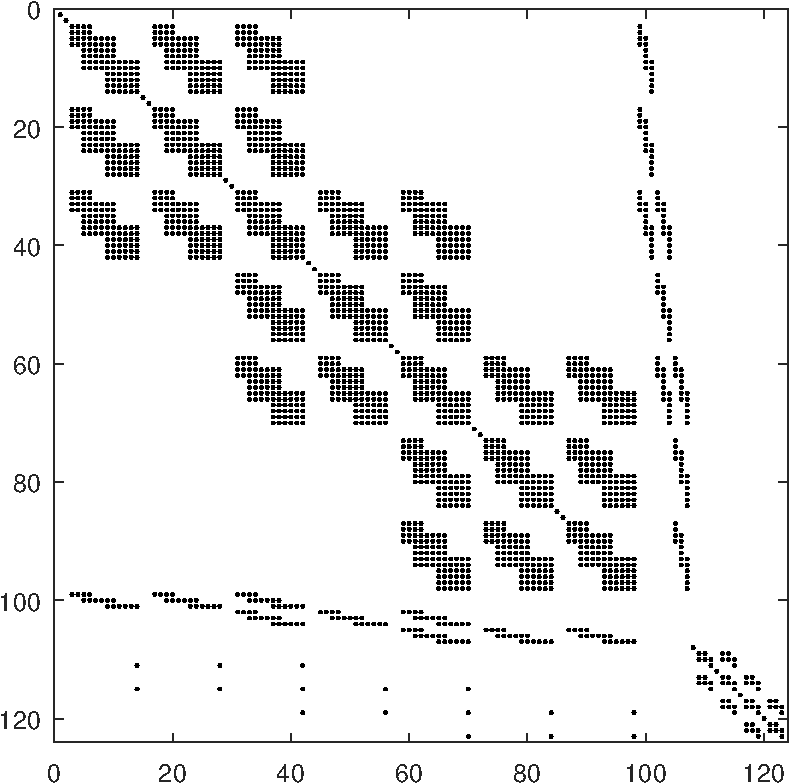
\includegraphics[width=0.5\textwidth]{coarsespy.pdf}
\end{center}
\caption{FIXME block structure of coupled problem}
\label{fig:blockstructure}
\end{figure}


\section{Inequality constraints and mass accounting} \label{sec:inequalities}

\begin{lemma}
Assume that the ice thickness is well defined at time $t_{n-1}$.  If [OLD] inequality holds then the updated ice surface elevation
    $$h(r) = \sup_{s\in I(r)}\{z(r,s)\}$$
satisfies \eqref{admissibility}, i.e.~$h(r)\ge b(r)$.
\end{lemma}

\begin{proof}
FIXME? This is the fundamental theorem of calculus:
    $$h(r) - b(r) = \int_{I(r)} 1\,ds \le \int_{I(r)} - \frac{\partial c}{\partial s}\,ds$$
\end{proof}


\section{Finite element approximation}  \label{sec:finiteelement}

FIXME: numerical solver should check element orientation under change of coordinates (above); if the solver flips an element then it is bad; also check new element aspect ratio and (presumably) remesh if that is bad; the initial iterate for the (SNES-based) solver is clear: $\bu,p$ come from solution of previous time step, and $b$ starts at zero

FIXME cite \cite{Tuminaroetal2016} re preconditioning for thin-film extruded meshes, and \cite{IsaacStadlerGhattas2015} for existing optimal Stokes solver for ice sheets

FIXME look back at Figure \ref{fig:blockstructure}


\section{Results}

FIXME among many things cite \cite{LeysingerGudmundsson2004} regarding earlier comparison of stokes to Halfar


\section{Discussion}

FIXME not appreciated that, while for explicit time-stepping schemes the surface mass balance need only be computed at the current ice surface, and at neighboring ice-free locations, in implicit time stepping the surface mass balance must be available to the evolving-geometry model (specifically to the residual-evaluation code) at every location in a 3D neighborhood of the ice surface, and indeed at all 3D locations above the bedrock elevation; a ``potential ice surface mass balance'' is needed at all such locations

\appendix
\section{The shallow ice approximation and its Halfar solutions}

In section FIXME, states of a certain similarity solution to an approximation of the Stokes problem are used as synthetic geometries for testing.  They arise from the $n=3$, isothermal, flat-bed ($b=0$), and zero surface mass balance ($a=0$) case of the shallow ice approximation.  This model, derived by \cite{GreveBlatter2009} among other sources, determines an evolving ice thickness function $H(t,x,y)$ according to a nonlinear, free-boundary diffusion which applies on the set where $H>0$:
\begin{equation}
\frac{\partial H}{\partial t} = \Gamma \Div \left(H^5 |\grad H|^2 \grad H\right). \label{sia}
\end{equation}
(References \cite{Bueler2016} and \cite{JouvetBueler2012} consider the rigorous meaning of this free boundary problem.)  In this equation we define $\Gamma = \frac{2}{5} A_3 (\rho g)^n$; constants $A_3,\rho,g$ have the same meaning and values as in the body of the paper.

P.~Halfar \cite{Halfar1981,Halfar1983} seems to have been the first to observe that \eqref{sia} has a similarity solution with $\lim_{t\to 0} H$ equal to a multiple of the Dirac delta function, and he observed that this solution is asymptotically stable.  This solution exactly solves the shallow approximation of no-slip flow.  Informally, the solution is a circular dome which spreads radially while thinning, with constant-in-time total volume.

In more detail, denoting the usual radial coordinate as $r=(x^2+y^2)^{1/2}$, the Halfar solution \cite{Halfar1983} is of the form $H(t,r) = t^{-\alpha} \varphi(s)$ with similarity variable $s=t^{-\beta} r$ and $\alpha=1/9$ and $\beta=1/18$.  If $H_0$ is a given central thickness value at a time $t_0$, and $R_0$ is a given radius, then the solution is
    $$H(t,x,y) = H_0 \left(\frac{t}{t_0}\right)^{-\alpha} \left\{1 - \left[\left(\frac{t}{t_0}\right)^{-\beta} \frac{r}{R_0}\right]^{4/3}\right\}^{3/7}.$$
This formula applies where the resulting value is positive, and $H=0$ otherwise; see \cite{Bueleretal2005}.  The characteristic time can by found by $\displaystyle t_0 = \frac{\beta}{\Gamma} \left(\frac{7}{4}\right)^3 \frac{R_0^4}{H_0^7}$.

The corresponding $d=2$ Halfar solution \cite{Halfar1981}, namely in one horizontal dimension, is of the form $H(t,x) = t^{-\alpha} \varphi(s)$ with similarity variable $s=t^{-\alpha} x$ and $\alpha=1/11$.  The solution is
    $$H(t,x) = H_0 \left(\frac{t}{t_0}\right)^{-\alpha} \left\{1 - \left[\left(\frac{t}{t_0}\right)^{-\alpha} \frac{x}{R_0}\right]^{4/3}\right\}^{3/7},$$
with characteristic time $\displaystyle t_0 = \frac{\alpha}{\Gamma} \left(\frac{7}{4}\right)^3 \frac{R_0^4}{H_0^7}$.

\small

\bigskip
\bibliography{simp}
\bibliographystyle{siam}

\end{document}
